% \documentclass[../main-physics-workbook.tex]{subfiles}

\documentclass[]{exam}
\usepackage{marvosym}

%...TikZ & PGF
\usepackage{pgfplots}
\pgfplotsset{compat=1.11}
\tikzset{>=latex}
\usetikzlibrary{calc,math}
\usepackage{tikzsymbols}
\usepgfplotslibrary{fillbetween}
\usetikzlibrary{decorations.markings} 
\usetikzlibrary{arrows.meta} %...APP2 for arrows as objects and images
\usetikzlibrary{backgrounds} %...For shading portions of graphs
\usetikzlibrary{patterns} %...Unit 5 Problems
\usetikzlibrary{shapes.geometric} %...For drawing cylinders in Unit 2
\usepackage{makecell} %...use \thead{} to enable line skip in table headers
\tikzset{
    mark position/.style args={#1(#2)}{
        postaction={
            decorate,
            decoration={
                markings,
                mark=at position #1 with \coordinate (#2);
            }
        }
    }
} %...See https://tex.stackexchange.com/questions/43960/define-node-at-relative-coordinates-of-draw-plot

\tikzset{
    declare function = {trajectoryequation10(\x,\vi,\thetai)= tan(\thetai)*\x - 10*\x^2/(2*(\vi*cos(\thetai))^2);},
    declare function = {trajectoryequation(\x,\vi,\thetai)= tan(\thetai)*\x - 9.8*\x^2/(2*(\vi*cos(\thetai))^2);},
    declare function = {patheq(\x,\yi,\vi,\thetai)= \yi + tan(\thetai)*\x - 9.8*\x^2/(2*(\vi*cos(\thetai))^2);},
    declare function = {patheqten(\x,\yi,\vi,\thetai)= \yi + tan(\thetai)*\x - 10*\x^2/(2*(\vi*cos(\thetai))^2);} %like patheq but with gravity = 10
}

%...siunitx
\usepackage{siunitx}
\DeclareSIUnit{\nothing}{\relax}
\def\mymu{\SI{}{\micro\nothing} }
\DeclareSIUnit\mmHg{mmHg}
\DeclareSIUnit{\mile}{mi}
%...NOTE: "The product symbol between the number and unit is set using the quantity-product option."

%...Other
\usepackage{amsthm}
\usepackage{amsmath}
\usepackage{amssymb}
\usepackage{cancel}
\usepackage{subcaption}
\usepackage{dashrule}
\usepackage{enumitem}
\usepackage{fontawesome}
\usepackage{multicol}
\usepackage{glossaries}
%\numberwithin{equation}{section}
\numberwithin{figure}{section}
\usepackage{float}
\usepackage{twemojis} %...twitter emojis
\usepackage{utfsym}
\usepackage{linearb} %...For \BPwheel in Unit 8
\newcommand{\R}{\mathbb{R}} %...real number symbol
\usepackage{graphicx}
\graphicspath{ {../Figures/} }
\usepackage{hyperref}
\hypersetup{colorlinks=true,
    linkcolor=blue,
    filecolor=magenta,
    urlcolor=cyan,}
\urlstyle{same}
\newcommand{\hdashline}{{\hdashrule{\textwidth}{0.5pt}{0.8mm}}}
\newcommand{\hgraydashline}{{\color{lightgray} \hdashrule{0.99\textwidth}{1pt}{0.8mm}}}

%...Miscellaneous user-defined symbols
\newcommand{\fnet}{F_{\text{net}}} %...For net force
\newcommand{\bvec}[1]{\vec{\mathbf{#1}}} %...bold vector
\newcommand{\bhat}[1]{\,\hat{\mathbf{#1}}} %...bold hat vector
\newcommand{\que}{\mathord{?}}  %...Question mark symbol in equation env
%...Define thick horizontal rule for examples:
\newcommand{\hhrule}{\hrule\hrule}
\let\oldtexttt\texttt% Store \texttt
\renewcommand{\texttt}[2][black]{\textcolor{#1}{\ttfamily #2}}% 

%...For use in the exam document class
\newif\ifprintmetasolutions


%...Decreases space above and below align and gather enironment
\makeatletter
\g@addto@macro\normalsize{%
  \setlength\abovedisplayskip{-3pt}
  \setlength\belowdisplayskip{6pt} 
}
\makeatother





\usepackage[margin=1in]{geometry}
\usepackage[figurewithin=none]{caption}
\usepackage{exam-randomizechoices}
\setrandomizerseed{1}

\CorrectChoiceEmphasis{\color{red}\bfseries}
\renewcommand{\solutiontitle}{\noindent\textbf{\textcolor{red}{Solution:}}\enspace}

\usepackage{OutilsGeomTikz}
\usepackage{utfsym} %...Symbols in Unit 7 Problems
\usepackage{tabu} %...Symbols in Unit 7 Problems

%...For use in Unit 2            %    
\setlength{\columnsep}{2cm}      %
\setlength{\columnseprule}{1pt}  %
\usepackage[none]{hyphenat}      %
%%%%%%%%%%%%%%%%%%%%%%%%%%%%%%%%%

%...For use in Unit 11 on Waves:
\pgfdeclarehorizontalshading{visiblelight}{50bp}{  %
color(0.00000000000000bp)=(red);                   %
color(8.33333333333333bp)=(orange);                %
color(16.66666666666670bp)=(yellow);               %
color(25.00000000000000bp)=(green);                %
color(33.33333333333330bp)=(cyan);                 %
color(41.66666666666670bp)=(blue);                 %
color(50.00000000000000bp)=(violet)                %
}                                                  %

\newcommand{\checkbox}[1]{%
  \ifnum#1=1
    \makebox[0pt][l]{\raisebox{0.15ex}{\hspace{0.1em}\Large$\checkmark$}}%
  \fi
  $\square$%
}
%%%%%%%%%%%%%%%%%%%%%%%%%%%%%%%%%%%%%%%%%%%%%%%%%%%%

%...If using circuitikz package:
% \ctikzset{bipoles/battery1/height=0.5}
% \ctikzset{bipoles/battery1/width=0.25}
% \ctikzset{bipoles/resistor/height=0.15}
% \ctikzset{bipoles/resistor/width=0.4}
\makenoidxglossaries

%...UNIT 1: CONSTANT MOTION

\newglossaryentry{scalar}{
    name=scalar,
    description={a quantity that has magnitude (and possibly sign) but no direction}
}

\newglossaryentry{magnitude}{
    name={magnitude},
    description={size or amount}
}

\newglossaryentry{vector}{
    name={vector},
    description={a quantity that has both magnitude and direction}
}

\newglossaryentry{tail}{
    name={tail},
    description={the starting point of a vector; the point opposite to the head or tip of the arrow}
}

\newglossaryentry{head}{
    name={head},
    description={the end point of a vector; the location of the vector's arrow; also referred to as the tip}
}

\newglossaryentry{head-to-tail method}{
    name={head-to-tail method},
    description={a method of adding vectors in which the tail of each vector is placed at the head of the previous vector}
}

\newglossaryentry{position}{
    name={position},
    description={the location of an object at any particular time}
}

\newglossaryentry{reference frame}{
    name={reference frame},
    description={a coordinate system from which the positions of objects are described}
}


\newglossaryentry{displacement}{
    name={displacement},
    description={the change in position of an object against a fixed axis}
}

\newglossaryentry{distance}{
    name={distance},
    description={the length of the path actually traveled between an initial and a final position}
}

\newglossaryentry{position vs. time graph}{
    name={position vs. time graph},
    description={a graph in which position is plotted on the vertical axis and time is plotted on the horizontal axis}
}

\newglossaryentry{speed}{
    name={speed},
    description={rate at which an object changes its location}
}

\newglossaryentry{average speed}{
    name={average speed},
    description={distance traveled divided by the time during which the motion occurs}
}

\newglossaryentry{velocity}{
    name={velocity},
    description={the speed and direction of an object}
}

\newglossaryentry{average velocity}{
    name={average velocity},
    description={displacement divided by the time during which the displacement occurs}
}

\newglossaryentry{velocity vs. time graph}{
    name={velocity vs. time graph},
    description={a graph in which velocity is plotted on the vertical axis and time is plotted on the horizontal axis}
}

\newglossaryentry{mass}{
    name=mass,
    description={the quantity of matter in a substance; the SI unit of mass is the kilogram}
}

\newglossaryentry{inertia}{
    name=inertia,
    description={the tendency of an object at rest to remain at rest, or for a moving object to remain in motion in a straight line and at a constant speed}
}

\newglossaryentry{Newton's first law of motion}{
    name={Newton's first law of motion},
    description={a body at rest remains at rest or, if in motion, remains in motion at a constant speed in a straight line, unless acted on by a net external force; also known as the law of inertia}
}

\newglossaryentry{momentum}{
    name={momentum},
    description={the product of a system's mass and velocity}
}

\newglossaryentry{momentum vs. time graph}{
    name={momentum vs. time graph},
    description={a graph in which momentum is plotted on the vertical axis and time is plotted on the horizontal axis}
}

\newglossaryentry{kinetic energy}{
    name={kinetic energy},
    description={energy of motion}
}

\newglossaryentry{joule}{
    name=joule,
    description={the metric unit for work and energy; equal to 1 newton meter ($\text{N}\cdot\text{m}$)}
}

\newglossaryentry{relative speed}{
    name={relative speed},
    description={how fast or slow an object appears to be moving to another object}
}

\newglossaryentry{relative velocity}{
    name={relative velocity},
    description={the rate at which an object changes position relative to another object}
}

%...UNIT 2: FORCE INTERACTIONS

\newglossaryentry{force}{
    name=force,
    description={a push or pull on an object with a specific magnitude and direction; can be represented by vectors; can be expressed as a multiple of a standard force; the SI unit of force is the Newton (N)}
}

\newglossaryentry{external force}{
    name=external force,
    description={a force acting on an object or system that originates outside of the object or system}
}

\newglossaryentry{free body diagram}{
    name=free body diagram,
    description={a diagram showing all external forces acting on a body}
}

\newglossaryentry{frictional force}{
    name=frictional force,
    description={an external force that acts opposite to the direction of motion or, for when there is no relative motion, in the direction needed to prevent slipping}
}

\newglossaryentry{applied force}{
    name={applied force},
    description={a contact force intentionally implied by a person on an object}
}


\newglossaryentry{gravitational force}{
    name=gravitational force, %...MY DEFINITION
    description={the downward force on an object due to the attraction by the Earth or other massive body}
}

\newglossaryentry{net force}{
    name=net force,
    description={the sum of all forces acting on an object or system}
}

\newglossaryentry{normal force}{
    name=normal force,
    description={that component of the contact force between two objects, which acts perpendicularly to and away from their plane of contact}
}

\newglossaryentry{tension}{
    name=tension,
    description={a pulling force that acts along a connecting medium, especially a stretched flexible connector, such as a rope or cable; when a rope supports the weight of an object, the force exerted on the object by the rope is called tension}
}

\newglossaryentry{spring force}{
    name=spring force, %...From district slides
    description={a force applied from a spring when it is either compressed or stretched}
}

%...UNIT 3: ACCELERATION

\newglossaryentry{acceleration}{
    name={acceleration},
    description={a change in velocity over time}
}

\newglossaryentry{average acceleration}{
    name={average acceleration},
    description={change in velocity divided by the time interval over which it changed}
}

%...UNIT 4:


\newglossaryentry{impulse}{
    name={impulse},
    description={average net external force multiplied by the time the force acts; equal to the change in momentum}
}

\newglossaryentry{impulse-momentum theorem}{
    name={impulse-momentum theorem},
    description={the impulse equals change in momentum}
}

\newglossaryentry{work}{
    name={work},
    description={force multiplied by distance}
}

%...UNIT 5: FORCE ANALYSIS

\newglossaryentry{Newton's universal law of gravitation}{
    name={Newton's universal law of gravitation},
    description={states that gravitational force between two objects is directly proportional to the product of their masses and inversely proportional to the square of the distance between them}
}

\newglossaryentry{gravitational constant}{
    name={gravitational constant},
    description={the proportionality constant in Newton's law of universal gravitation}
}

\newglossaryentry{weight}{
    name={weight},
    description={the force of gravity, $W$, acting on an object of mass $m$; defined mathematically as $W = mg$, where $g$ is the acceleration due to gravity}
}

\newglossaryentry{contact force}{
    name={contact force},
    description={a type of force that occurs when objects are physically in contact with each other}
}

%...UNIT 6: ONE-DIMENSIONAL MOTION

\newglossaryentry{free fall}{
    name=free fall,
    description={a situation in which the only force acting on an object is the force of gravity}
}

\newglossaryentry{kinematic equations}{
    name={kinematic equations},
    description={the 
    %five 
    equations that describe constant acceleration motion in terms of time, displacement, velocity, and acceleration}
}

%...UNIT 7: MOTION IN TWO DIMENSIONS

\newglossaryentry{projectile}{
    name={projectile},
    description={an object that travels through the air and experiences only acceleration due to gravity}
}

\newglossaryentry{projectile motion}{
    name={projectile motion},
    description={the motion of an object that is subject only to the acceleration of gravity}
}

\newglossaryentry{trajectory}{
    name={trajectory},
    description={the path of a projectile through the air}
}

\newglossaryentry{apex}{
    name={apex},
    description={the location on the trajectory at which the projectile reaches maximum height}
}

\newglossaryentry{hang time}{
    name={hang time},
    description={the amount of time that a projectile is in the air during projectile motion}
}

\newglossaryentry{horizontally launched projectile}{
    name={horizontally launched projectile},
    description={a projectile whose initial velocity is entirely in the horizontal direction}
}

\newglossaryentry{impact speed}{
    name={impact speed},
    description={the speed at which a projectile strikes the ground after being launched}
}

%...UNIT 8: CONSERVATION IN MECHANICAL SYSTEMS

\newglossaryentry{system}{
    name={system},
    description={one or more objects of interest for which only the forces acting on them from the outside are considered, but not the forces acting between them or inside them}
}

\newglossaryentry{energy}{
    name={energy},
    description={the ability to do work}
}

\newglossaryentry{potential energy}{
    name={potential energy},
    description={stored energy}
}

\newglossaryentry{gravitational potential energy}{
    name={gravitational potential energy},
    description={energy acquired by doing work against gravity}
}

\newglossaryentry{law of conservation of energy}{
    name={law of conservation of energy},
    description={states that energy is neither created nor destroyed}
}

\newglossaryentry{mechanical energy}{
    name={mechanical energy},
    description={kinetic plus potential energy}
}

\newglossaryentry{elastic collision}{
    name={elastic collision},
    description={a collision in which objects separate after impact and kinetic energy is conserved}
}

\newglossaryentry{inelastic collision}{
    name={inelastic collision},
    description={a collision in which kinetic energy is not conserved}
}

\newglossaryentry{isolated system}{
    name={isolated system},
    description={system in which the net external force is zero}
}

\newglossaryentry{law of conservation of momentum}{
    name={law of conservation of momentum},
    description={when the net external force is zero, the total momentum of the system is conserved or constant}
}

\newglossaryentry{perfectly inelastic collision}{
    name={perfectly inelastic collision},
    description={collision in which objects stick together after impact and kinetic energy is not conserved}
}

\newglossaryentry{recoil}{
    name={recoil},
    description={backward movement of an object caused by the transfer of momentum from another object in a collision}
}

%...UNIT 9: CONSERVATION OF CHARGE

\newglossaryentry{electric charge}{
    name={electric charge},
    description={a physical property of an object that causes it to be attracted toward or repelled from another charged object; each charged object generates and is influenced by a force called an electromagnetic force}
}

\newglossaryentry{elementary charge}{
    name={elementary charge},
    description={the smallest observed unit of charge that can be isolated in nature; also, the magnitude of charge on 1 proton or 1 electron}
}

\newglossaryentry{electron}{
    name={electron},
    description={subatomic particle that carries one indivisible unit of negative electric charge}
}

\newglossaryentry{proton}{
    name={proton},
    description={subatomic particle that carries the same magnitude charge as the electron, but its charge is positive}
}

\newglossaryentry{electric field}{
    name={electric field},
    description={defines the force per unit charge at all locations in space around a charge distribution}
}

\newglossaryentry{law of conservation of charge}{
    name={law of conservation of charge},
    description={states that total charge is constant in any process}
}

\newglossaryentry{polarization}{
    name={polarization},
    description={separation of charge induced by nearby excess charge}
}

\newglossaryentry{Coulomb's law}{
    name={Coulomb's law},
    description={describes the electrostatic force between charged objects, which is proportional to the charge on each object and inversely proportional to the square of the distance between the objects}
}

\newglossaryentry{electric circuit}{
    name={electric circuit},
    description={physical network of paths through which electric current can flow}
}

\newglossaryentry{simple circuit}{
    name={simple circuit},
    description={a circuit with a single voltage source and a single resistor}
}

\newglossaryentry{electric current}{
    name={electric current},
    description={electric charge that is moving}
}


\newglossaryentry{Ohm's law}{
    name={Ohm's law},
    description={electric current is proportional to the voltage applied across a circuit or other path}
}

\newglossaryentry{resistance}{
    name={resistance},
    description={how much a circuit element opposes the passage of electric current; it appears as the constant of proportionality in Ohm’s law}
}

\newglossaryentry{resistor}{
    name={resistor},
    description={circuit element that provides a known resistance}
}

% \newglossaryentry{potential difference (or voltage)}{
%     name={potential difference (or voltage)},
%     description={change in potential energy of a charge moved from one point to another, divided by the charge; units of potential difference are joules per coulomb, known as volt}
% }

\newglossaryentry{voltage}{
    name={voltage},
    description={the electrical potential energy per unit charge; electric pressure created by a power source, such as a battery}
}

\newglossaryentry{electric power}{
    name={electric power},
    description={rate at which electric energy is transferred in a circuit}
}

\newglossaryentry{equivalent resistor}{
    name={equivalent resistor},
    description={resistance of a single resistor that is the same as the combined resistance of a group of resistors}
}

\newglossaryentry{in series}{
    name={in series},
    description={when elements in a circuit are connected one after the other in the same branch of the circuit}
}

\newglossaryentry{in parallel}{
    name={in parallel},
    description={when a group of resistors are connected side by side, with the top ends of the resistors connected together by a wire and the bottom ends connected together by a different wire}
}

\newglossaryentry{induction}{
    name={induction},
    description={creating an unbalanced charge distribution in an object by moving a charged object toward it (but without touching)}
}

%...UNIT 10: ELECTROMAGNETIC INDUCTION

\newglossaryentry{magnetic dipole}{
    name={magnetic dipole},
    description={term that describes magnets because they always have two poles: north and south}
}

\newglossaryentry{magnetic field}{
    name={magnetic field},
    description={directional lines around a magnetic material that indicates the direction and magnitude of the magnetic force}
}

\newglossaryentry{magnetic pole}{
    name={magnetic pole},
    description={part of a magnet that exerts the strongest force on other magnets or magnetic material}
}

\newglossaryentry{electromagnetic induction}{
    name={electromagnetic induction},
    description={rate at which energy is drawn from a source per unit current flowing through a circuit}
}


\newglossaryentry{Faraday's law}{
    name={Faraday's law},
    description={the means of calculating the emf in a coil due to changing magnetic flux}
}

\newglossaryentry{electromagnet}{
    name={electromagnet},
    description={device that uses electric current to make a magnetic field}
}

\newglossaryentry{transformer}{
    name={transformer},
    description={device that transforms voltages from one value to another}
}

\newglossaryentry{electric motor}{
    name={electric motor},
    description={device that transforms electrical energy into mechanical energy}
}

\newglossaryentry{generator}{
    name={generator},
    description={device that transforms mechanical energy into electrical energy}
}

%...UNIT 11: SIMPLE HARMONIC MOTION & WAVES

\newglossaryentry{wave}{
    name={wave},
    description={a disturbance that moves from its source and carries energy}
}

\newglossaryentry{wave velocity}{
    name={wave velocity},
    description={speed at which the disturbance moves; also called the propagation velocity or propagation speed}
}

\newglossaryentry{wavelength}{
    name={wavelength},
    description={distance between adjacent identical parts of a wave}
}

\newglossaryentry{wave cycle}{
    name={wave cycle},
    description={any portion of a wave encompassed by 1 wavelength}
}

\newglossaryentry{transverse wave}{
    name={transverse wave},
    description={a wave in which the disturbance is perpendicular to the direction of propagation}
}

\newglossaryentry{medium}{
    name={medium},
    description={the solid, liquid, or gas material through which a wave propagates}
}

\newglossaryentry{mechanical wave}{
    name={mechanical wave},
    description={wave that requires a medium through which it can travel}
}

\newglossaryentry{longitudinal wave}{
    name={longitudinal wave},
    description={wave in which the disturbance is parallel to the direction of propagation}
}

\newglossaryentry{constructive interference}{
    name={constructive interference},
    description={when two waves arrive at the same point exactly in phase; that is, the crests of the two waves are precisely aligned, as are the troughs}
}

\newglossaryentry{destructive interference}{
    name={destructive interference},
    description={when two identical waves arrive at the same point exactly out of phase that is precisely aligned crest to trough}
}

\newglossaryentry{oscillate}{
    name={oscillate},
    description={to move back and forth regularly between two points}
}

\newglossaryentry{amplitude}{
    name={amplitude},
    description={the maximum displacement from the equilibrium position of an object oscillating around the equilibrium position}
}

\newglossaryentry{frequency}{
    name={frequency},
    description={number of wave cycles per unit of time}
}

\newglossaryentry{simple harmonic motion}{
    name={simple harmonic motion},
    description={the oscillatory motion in a system where the net force can be described by Hooke’s law}
}

\newglossaryentry{simple harmonic oscillator}{
    name={simple harmonic oscillator},
    description={a device that oscillates in SHM,  such as a mass that is attached to a spring, where the restoring force is proportional to the displacement and acts in the direction opposite to the displacement}
}

\newglossaryentry{period}{
    name={period},
    description={the time it takes to complete one oscillation}
}

\newglossaryentry{electromagnetic wave}{
    name={electromagnetic wave},
    description={a radiant energy wave that consists of oscillating electric and magnetic fields}
}

\newglossaryentry{electromagnetic radiation}{
    name={electromagnetic radiation},
    description={radiant energy that consists of oscillating electric and magnetic fields}
}









%... Overview and Student Learning Expectations (OSLE)

\newglossaryentry{OSLE 6.1.a}{
    name={OSLE 6.1.a},
    description={compare the gravitational field strength on Earth to the acceleration due to gravity on Earth}
}

\newglossaryentry{OSLE 6.1.b}{
    name={OSLE 6.1.b},
    description={explain using universal gravitation and $F_\mathrm{net}=ma$ why all objects near Earth's surface fall at the same rate when in free fall}
}

\newglossaryentry{OSLE 6.1.c}{
    name={OSLE 6.1.c},
    description={explain the relationship between the mass, initial position, and initial velocity of an object in free fall on its final velocity and/or time in free fall}
}

\newglossaryentry{OSLE 6.1.d}{
    name={OSLE 6.1.d},
    description={describe the displacement, velocity, momentum, kinetic energy, and acceleration of an object in free fall that was dropped, thrown upward, or thrown downward using Multiple Representations}
}

\newglossaryentry{OSLE 6.1.e}{
    name={OSLE 6.1.e},
    description={relate the gravitational force, impulse, and work done on the object by the Earth to the object's change in velocity (acceleration), momentum, and kinetic energy}
}

        
\newglossaryentry{OSLE 6.2.a}{
    name={OSLE 6.2.a},
    description={describe what is known about an object's motion in a constant acceleration word problem using Multiple Representations}
}

\newglossaryentry{OSLE 6.2.b}{
    name={OSLE 6.2.b},
    description={solve for various unknown quantities utilizing kinematic equations when data is given in Multiple Representations for objects moving horizontally with constant acceleration}
}

\newglossaryentry{OSLE 6.3.c}{
    name={OSLE 6.3.c},
    description={solve for various unknown quantities utilizing kinematic equations when data is given in Multiple Representations for objects moving vertically with constant acceleration (free fall)}
}

\newglossaryentry{OSLE 6.4.d}{
    name={OSLE 6.4.d},
    description={solve multi-step problems that connect kinematic equations, the Law of Acceleration, Work-Energy Theorem, and/or the Impulse-Momentum Theorem}
}

\newglossaryentry{OSLE 7.1.a}{
    name={OSLE 7.1.a},
    description={compare the trajectory, hang time, max height, range, and final velocity of various projectiles that have different initial velocities, launch heights, launch angles, and masses, only varying one parameter at a time}
}

\newglossaryentry{OSLE 7.1.b}{
    name={OSLE 7.1.b},
    description={identify if and explain how the  initial velocity, launch height, launch angle, and mass of a projectile influence its motion---hang time, height, range, final velocity}
}

\newglossaryentry{OSLE 7.2.a}{
    name={OSLE 7.2.a},
    description={describe the vertical and horizontal motion of a projectile with a launch angle of zero using Multiple Representations}
}

\newglossaryentry{OSLE 7.2.b}{
    name={OSLE 7.2.b},
    description={illustrate the resultant motion of the projectile at any point in its trajectory as well as the relationship between the horizontal and vertical components using vector addition}
}

\newglossaryentry{OSLE 7.2.c}{
    name={OSLE 7.2.c},
    description={analyze and solve word problems about the motion of  horizontally launched projectiles using kinematic equations, vector addition, and  Multiple Representations}
}

\newglossaryentry{OSLE 7.3.a}{
    name={OSLE 7.3.a},
    description={describe the motion of an object moving with uniform circular motion in terms of centripetal force, centripetal acceleration, momentum, kinetic energy, and tangential velocity using Multiple Representations}
}

\newglossaryentry{OSLE 7.3.b}{
    name={OSLE 7.3.b},
    description={determine the centripetal force, mass, centripetal acceleration, tangential velocity, or radius of an object in circular motion}
}

\newglossaryentry{OSLE 7.4.a}{
    name={OSLE 7.4.a},
    description={predict the effects of changing the radius or mass of objects in orbiting systems using concepts of uniform circular motion and Newton’s law of universal gravitation}
}


\newglossaryentry{OSLE 8.1.a}{
    name={OSLE 8.1.a},
    description={identify multiple choices for a system given a scenario}
}

\newglossaryentry{OSLE 8.1.b}{
    name={OSLE 8.1.b},
    description={recognize that energy can be stored in the arrangement of particles or objects in a system as potential energy}
}

\newglossaryentry{OSLE 8.1.c}{
    name={OSLE 8.1.c},
    description={identify and calculate (i) gravitational potential energy and (ii) elastic potential energy when a system includes energy stored in the arrangement of its particles or objects}
}

\newglossaryentry{OSLE 8.1.d}{
    name={OSLE 8.1.d},
    description={compare the potential energy of a scenario for various choices of system}
}

\newglossaryentry{OSLE 8.1.e}{
    name={OSLE 8.1.e},
    description={identify, represent using multiple representations, and calculate the total mechanical energy present in a physical system}
}

\newglossaryentry{OSLE 8.1.f}{
    name={OSLE 8.1.f},
    description={predict the effects of changing the mass, velocity, height, gravitational field strength, spring constant, compression or stretching distance on the amount of $E_k$, $E_\mathrm{GP}$, and $E_\mathrm{SP}$}
}

\newglossaryentry{OSLE 8.1.g}{
    name={OSLE 8.1.g},
    description={calculate the total mechanical energy of a system}
}

\newglossaryentry{OSLE 8.2.a.i}{
    name={OSLE 8.2.a.i},
    description={identify, represent using multiple representations, and calculate the amount of energy (1) transformed from one storage mode to another within a system (including kinetic energy, potential energy, and thermal energy), (2) transferred from one object in the system to another in the system, and (3) entering/leaving a system due to work, heat, light, or sound}
}

\newglossaryentry{OSLE 8.2.b.i}{
    name={OSLE 8.2.b.i},
    description={explain the meaning of the Law of Conservation of Energy}
}

\newglossaryentry{OSLE 8.2.b.ii}{
    name={OSLE 8.2.b.ii},
    description={develop an energy formula for systems using energy bar charts and the Law of Conservation of Energy}
}

\newglossaryentry{OSLE 8.2.b.iii}{
    name={OSLE 8.2.b.iii},
    description=solve for various unknown quantities using the concept of the conservation of energy{}
}

\newglossaryentry{OSLE 8.2.c.i}{
    name={OSLE 8.2.c.i},
    description={know the definition of work as change in energy of a system}
}

\newglossaryentry{OSLE 8.2.c.ii}{
    name={OSLE 8.2.c.ii},
    description={know that power is work done divided by time}
}

\newglossaryentry{OSLE 8.3.a}{
    name={OSLE 8.3.a},
    description={calculate and compare the momentum, changes in momentum, force applied to and impulse on each object involved in a collision or explosion scenario}
}

\newglossaryentry{OSLE 8.3.b}{
    name={OSLE 8.3.b},
    description={represent using multiple representations, compare, and calculate the total momentum of a system before and after a collision or explosion scenario}
}

\newglossaryentry{OSLE 8.3.c}{
    name={OSLE 8.3.c},
    description={explain the meaning of the Law of Conservation of Momentum}
}

\newglossaryentry{OSLE 8.3.d}{
    name={OSLE 8.3.d},
    description={solve for unknown quantities using the concept of the conservation of momentum}
}


\newglossaryentry{OSLE 9.1.a}{
    name={OSLE 9.1.a},
    description={identify the particles that contribute positive, negative, or no charge in an atom}
}

\newglossaryentry{OSLE 9.1.b}{
    name={OSLE 9.1.b},
    description={recognize that neutral objects have even numbers of positive and negative charges}
}

\newglossaryentry{OSLE 9.1.c}{
    name={OSLE 9.1.c},
    description={determine the charge of an object given the number of protons and electrons}
}

\newglossaryentry{OSLE 9.1.d}{
    name={OSLE 9.1.d},
    description={predict if two objects will attract, repel, or have no interaction based on their charges}
}

\newglossaryentry{OSLE 9.1.e}{
    name={OSLE 9.1.e},
    description={draw the electric field surrounding single charges and pairs of charges}
}

\newglossaryentry{OSLE 9.2.a}{
    name={OSLE 9.2.a},
    description={recognize that charge is conserved: it cannot be created or destroyed, only transferred}
}

\newglossaryentry{OSLE 9.2.b}{
    name={OSLE 9.2.b},
    description={realize that only electrons are transferred during charging}
}

\newglossaryentry{OSLE 9.2.c}{
    name={OSLE 9.2.c},
    description={compare and contrast charging by induction and conduction}
}

\newglossaryentry{OSLE 9.2.d}{
    name={OSLE 9.2.d},
    description={explain how polarization temporarily charges a neutral object}
}

\newglossaryentry{OSLE 9.2.e}{
    name={OSLE 9.2.e},
    description={describe how an electroscope determines if objects are charged}
}

\newglossaryentry{OSLE 9.2.f}{
    name={OSLE 9.2.f},
    description={determine whether an object is negatively charged, positively charged, or neutral when given the charge of one object and a description or diagram representing how the charged object interacts with an object of unknown charge}
}

\newglossaryentry{OSLE 9.2.g}{
    name={OSLE 9.2.g},
    description={draw and describe the resulting distribution of charge for various scenarios of induction, conduction, and polarization}
}


\newglossaryentry{OSLE 9.3.a}{
    name={OSLE 9.3.a},
    description={draw the free body diagram for 2 charged objects showing the direction and relative magnitude of the electrical force acting on each object at various distances from each other}
}

\newglossaryentry{OSLE 9.3.b}{
    name={OSLE 9.3.b},
    description={describe how the electric force depends on the charges and the distance between them}
}

\newglossaryentry{OSLE 9.3.c}{
    name={OSLE 9.3.c},
    description={compare and contrast the electric force to the gravitational force}
}

\newglossaryentry{OSLE 9.3.d}{
    name={OSLE 9.3.d},
    description={predict how changing the charge or distance affects the electric force}
}


\newglossaryentry{OSLE 9.4.a}{
    name={OSLE 9.4.a},
    description={identify the necessary components for a simple circuit and discover different ways to light a bulb}
}

\newglossaryentry{OSLE 9.4.b}{
    name={OSLE 9.4.b},
    description={trace the conducting path through a simple circuit}
}

\newglossaryentry{OSLE 9.4.c}{
    name={OSLE 9.4.c},
    description={explain the concepts of current, resistance, voltage}
}

\newglossaryentry{OSLE 9.4.d}{
    name={OSLE 9.4.d},
    description={measure the current, resistance and voltage in a circuit using a multimeter, ammeter, current probe, etc}
}

\newglossaryentry{OSLE 9.4.e}{
    name={OSLE 9.4.e},
    description={calculate the voltage drop across, current through, or resistance of a circuit component using Ohm’s Law}
}

\newglossaryentry{OSLE 9.4.f}{
    name={OSLE 9.4.f},
    description={determine the change in current as the voltage or resistance is changed}
}

\newglossaryentry{OSLE 9.4.g}{
    name={OSLE 9.4.g},
    description={interpret electrical power as the rate at which electrical energy is being dissipated in the circuit}
}

\newglossaryentry{OSLE 9.4.h}{
    name={OSLE 9.4.h},
    description={relate the power rating/wattage of a light bulb to its brightness}
}


\newglossaryentry{OSLE 9.5.a}{
    name={OSLE 9.5.a},
    description={measure the current, resistance and voltage at various locations in a series circuit using a multimeter, ammeter, current probe, etc}
}

\newglossaryentry{OSLE 9.5.b}{
    name={OSLE 9.5.b},
    description={describe qualitatively and quantitatively the current flow throughout a series circuit}
}

\newglossaryentry{OSLE 9.5.c}{
    name={OSLE 9.5.c},
    description={calculate the equivalent resistance of multiple resistors in series}
}

\newglossaryentry{OSLE 9.5.d}{
    name={OSLE 9.5.d},
    description={calculate the equivalent voltage of batteries in series}
}

\newglossaryentry{OSLE 9.5.e}{
    name={OSLE 9.5.e},
    description={recognize that the sum of the voltage drops across resistors in series equals the total voltage of the power supply}
}

\newglossaryentry{OSLE 9.5.f}{
    name={OSLE 9.5.f},
    description={describe the energy transformations (transfers) occurring in a series circuit}
}

\newglossaryentry{OSLE 9.5.g}{
    name={OSLE 9.5.g},
    description={determine (i) current through, voltage drop across, and power of each component, and (i) total current of circuit, when given a series circuit diagram}
}


\newglossaryentry{OSLE 9.6.a}{
    name={OSLE 9.6.a},
    description={measure the current, resistance and voltage at various locations in a parallel circuit using a multimeter, ammeter, current probe, etc}
}

\newglossaryentry{OSLE 9.6.b}{
    name={OSLE 9.6.b},
    description={recognize that the current going into a junction is equal to the current coming out of it}
}

\newglossaryentry{OSLE 9.6.c}{
    name={OSLE 9.6.c},
    description={describe qualitatively and quantitatively the current flow throughout a parallel circuit}
}

\newglossaryentry{OSLE 9.6.d}{
    name={OSLE 9.6.d},
    description={recognize that the voltage drops across each resistor are equal to the voltage of the power supply}
}

\newglossaryentry{OSLE 9.6.e}{
    name={OSLE 9.6.e},
    description={describe advantages and disadvantages of parallel circuits compared to series circuits}
}

\newglossaryentry{OSLE 9.6.f}{
    name={OSLE 9.6.f},
    description={calculate the equivalent resistance of multiple resistors in parallel}
}

\newglossaryentry{OSLE 9.6.g}{
    name={OSLE 9.6.g},
    description={calculate the equivalent voltage of batteries in parallel}
}

\newglossaryentry{OSLE 9.6.h}{
    name={OSLE 9.6.h},
    description={describe the energy transformations (transfers) occurring in a parallel circuit}
}

\newglossaryentry{OSLE 9.6.i}{
    name={OSLE 9.6.i},
    description={determine the (i) current through, voltage drop across, and power of each component, and (ii) total current of circuit, when given a series circuit diagram}
}


\newglossaryentry{OSLE 9.7.a}{
    name={OSLE 9.7.a},
    description={determine whether elements of a combination circuit have the same current or voltage}
}

\newglossaryentry{OSLE 9.7.b}{
    name={OSLE 9.7.b},
    description={predict which bulbs will light if switches are open or closed}
}







\usepackage{makecell}

\setcounter{section}{10}

\begin{document}





\subsection{PhET Simulation: Magnets and Electromangets}

\textbf{Directions:} Go to the \href{https://phet.colorado.edu/sims/html/magnets-and-electromagnets/latest/magnets-and-electromagnets_all.html}{PhET Simulation: Magnets and Electromagnets}.

\begin{questions}
\question
Click on the panel called Bar Magnet. Click the reset ($\circlearrowleft$) button in the bottom right corner. By default, the magnetic field and compass are enabled. Check the field meter box, too:

\begin{center}
    \checkbox{1} Magnetic Field (B) \qquad
    \checkbox{1} Compass \qquad
    \checkbox{1} Field Meter
\end{center}

\begin{center}
\ifprintanswers
\begin{tikzpicture}
    \node at (0,0) {\fcolorbox{red}{white}{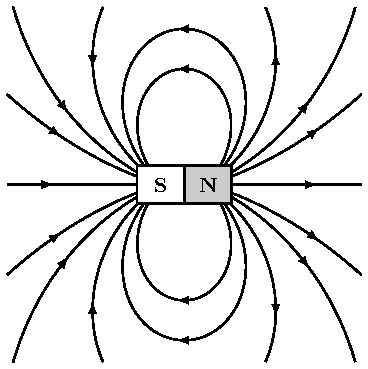
\includegraphics[width=5cm]{documents/figures/magnetic-field-lines-1.pdf}}};
\end{tikzpicture}
\else
\vspace{2cm}
\begin{tikzpicture}
    \fill[white] (-2,-0.4) rectangle (0,0.4);
    \fill[black!20] (0,-0.4) rectangle (2,0.4);
    \draw[rounded corners] (-2,-0.4) node[shift={(0.3,0.4)}] {\Large S} rectangle (2,0.4) node[shift={(-0.3,-0.4)}] {\Large N};
    \draw (0,-0.4) -- (0,0.4);
    \draw (3.1,-1.8) node {\rotatebox{-120}{\resizebox{10mm}{!}{\faCompass}}};
    \draw[<-,thick] (3.23,-1.85) -- ++(0.8,-0.4) node[right] {B};
    \draw (-4.9,-1.8) node {\resizebox{7mm}{!}{\faCrosshairs}} node[below=1em] {A};
    \fill (0,-0.5) circle (1.5pt) node[below=1.5pt] {\footnotesize C};
    \fill (0,0) circle (1.5pt) node[right=1pt] {\footnotesize D};
\end{tikzpicture}
\fi
    
\end{center}

\begin{parts}
\part Four points, A--D, are labeled for reference in the figure above.

\begin{itemize}
    \item Point A: the initial position of the field meter
    \item Point B: the center of the initial position of the compass
    \item Point C: the point below and just outside the magnet
    \item Point D: the midpoint inside the magnet
\end{itemize}

Use the field meter measure and record the magnetic field at the four points below:

\begin{equation*}
    B_\mathrm{A} = {\ifprintanswers \color{red} \else \color{white} \fi \SI{0.60}{G}} \hspace{1.3cm}
    B_\mathrm{B} = {\ifprintanswers \color{red} \else \color{white} \fi \SI{1.71}{G}} \hspace{1.3cm}
    B_\mathrm{C} = {\ifprintanswers \color{red} \else \color{white} \fi \SI{4.11}{G}} \hspace{1.3cm}
    B_\mathrm{D} = {\ifprintanswers \color{red} \else \color{white} \fi \SI{220.63}{G}} \hspace{1.3cm}
\end{equation*}

\medskip

\part In the space provided above, draw the magnetic field lines surrounding the magnet. Use the compass for guidance, and arrows to indicate the direction of the field lines.

\part Click the reset ($\circlearrowleft$) button and check the Earth box: \checkbox{1} Earth. Our home planet is a magnet, because it is surrounded by magnetic field lines. In the space below, \textbf{draw} the bar magnet, correctly labeling north and south magnetic poles, and \textbf{draw} the magnetic field lines surrounding the planet.

\begin{center}
\begin{tikzpicture}
    \ifprintanswers
    \node at (0,0) {\rotatebox{-90}{\fcolorbox{red}{white}{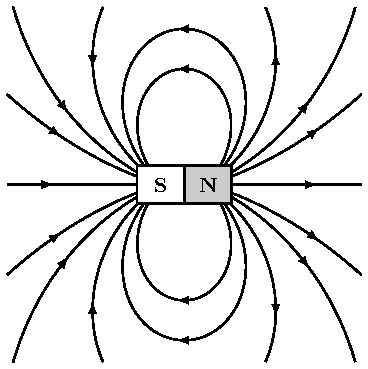
\includegraphics[width=7.4cm]{documents/figures/magnetic-field-lines-1.pdf}}}};
    \node at (0,0) {\twemoji[width=3.2cm]{globe showing Americas}};
    \else
    \node[opacity=0] at (0,0) {\rotatebox{-90}{\fcolorbox{red}{white}{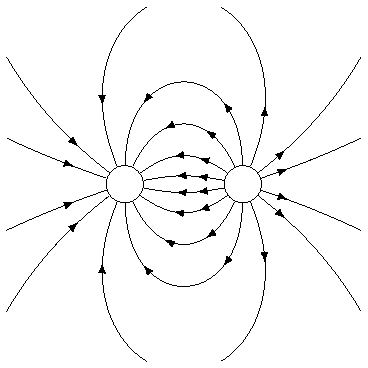
\includegraphics[width=7.4cm]{documents/figures/electric-field-lines-5a.pdf}}}};
    \node[opacity=0.5] at (0,0) {\twemoji[width=3.2cm]{globe showing Americas}};
    \fi
\end{tikzpicture}
\end{center}
\end{parts}

\clearpage

\question
Switch to the panel called Electromagnet (see the bar at the bottom of the screen). Check all the boxes:

\begin{center}
    \checkbox{1} Magnetic Field (B) \qquad
    \checkbox{1} Electrons \qquad
    \checkbox{1} Compass \qquad
    \checkbox{1} Field Meter
\end{center}

\begin{parts}
\part Read the field meter to record the magnetic field strength at the locations below:

\begin{itemize}[itemsep=6pt,topsep=4pt]
    \item The magnetic field at the initial position of the field meter is \fillin[\SI{1.44}{G}].
    \item The magnetic field at the center of the initial position of the compass is \fillin[\SI{2.65}{G}].
    \item The magnetic field inside the 4-coil electromagnet is \fillin[\SI{300.00}{G}].
\end{itemize}

\part Use the field meter to measure the magnetic field inside the electromagnetic coil as a function of the voltage in the battery. Record your data in the table and graph below.

\begin{EnvUplevel}
\begin{center}
% \fbox{
\begin{minipage}{6cm}
\centering
\bgroup
\def\arraystretch{1.15}
\begin{tabular}{|c|c|}
    \hline
    \thead{\textbf{Battery}\\ \textbf{Voltage} (V)} & \thead{\textbf{Magnetic}\\ \textbf{Field} (G)} \\ \hline
    $-5$ & {\ifprintanswers \color{red} 150 \fi} \\ \hline
    $-4$ & {\ifprintanswers \color{red} 120 \fi} \\ \hline
    $-3$ & {\ifprintanswers \color{red} 90 \fi} \\ \hline
    $-2$ & {\ifprintanswers \color{red} 60 \fi} \\ \hline
    $-1$ & {\ifprintanswers \color{red} 30 \fi} \\ \hline
    $0$ & {\ifprintanswers \color{red} 0.00 \fi} \\ \hline
    $1$ & {\ifprintanswers \color{red} 30 \fi} \\ \hline
    $2$ & {\ifprintanswers \color{red} 60 \fi} \\ \hline
    $3$ & {\ifprintanswers \color{red} 90 \fi} \\ \hline
    $4$ & {\ifprintanswers \color{red} 120 \fi} \\ \hline
    $5$ & {\ifprintanswers \color{red} 150 \fi} \\ \hline
\end{tabular}
\egroup
\end{minipage}
% }
% \fbox{
\begin{minipage}{8.5cm}
\centering
\begin{tikzpicture}
    \begin{axis}[height=6cm,
        width=8.5cm,
        axis y line=center,
        axis x line=left,
        ylabel={Magnetic Field (G)},
        xlabel={Battery Voltage (V)},
        y label style={at={(axis description cs: 0.5,1)},above=0.5em},
        x label style={at={(axis description cs: 0.7,0)},below=1.5em},
        ymin=0,ymax=180,
        xmin=-5,xmax=5,
        ytick={0,30,...,180},
        xtick={-5,-4,...,5},
        grid=both,
        % minor y tick num=1,
        % minor x tick num=1,
    ]
        \ifprintanswers
            \addplot[thick,red,mark=*,domain=-5:0,samples=6] {-30*x};
            \addplot[thick,red,mark=*,domain=0:5,samples=6] {30*x};
        \else
        \fi
    \end{axis}
\end{tikzpicture}
\end{minipage}
% }
\end{center}
\end{EnvUplevel}


\part Click the reset ($\circlearrowleft$) button, and check \checkbox{1} Field Meter. Set the loops number to 1, and measure the magnetic field inside the coil. Then increase the loop number, and fill the table and graph below.

\begin{EnvUplevel}
\begin{center}
% \fbox{
\begin{minipage}{5cm}
\centering
\bgroup
\def\arraystretch{1.2}
\begin{tabular}{|c|c|}
    \hline
    \thead{\textbf{Number}\\ \textbf{of Loops}} & \thead{\textbf{Magnetic}\\ \textbf{Field} (G)} \\ \hline
    1 & {\ifprintanswers \color{red} 75.00 \fi} \\ \hline
    2 & {\ifprintanswers \color{red} 150.00 \fi} \\ \hline
    3 & {\ifprintanswers \color{red} 225.00 \fi} \\ \hline
    4 & {\ifprintanswers \color{red} 300.00 \fi} \\ \hline
\end{tabular}
\egroup
\end{minipage}
% }
% \fbox{
\begin{minipage}{7.5cm}
\centering
\begin{tikzpicture}
    \begin{axis}[height=6cm,
        width=6cm,
        axis lines=left,
        ylabel={Magnetic Field (G)},
        xlabel={Number of Loops},
        ymin=0,ymax=300,
        xmin=0,xmax=4,
        ytick={0,60,...,300},
        xtick={0,1,...,4},
        grid=both,
        minor y tick num=1,
        minor x tick num=1,
    ]
        \ifprintanswers
        \addplot[thick,red,mark=*,domain=1:4,samples=4] {75*x};
        \else
        \fi
    \end{axis}
\end{tikzpicture}
\end{minipage}
% }
\end{center}
\end{EnvUplevel}

\part Numerically, what happens to the magnetic field in the coil when one loop is added to the electromagnet?

\begin{solution}
    Magnetic field increases by \SI{75}{G} with each loop.
\end{solution}

\fillwithlines{0.7cm}


\part \textit{Predict:} What would be the strength of the magnetic field inside the coil if there were 9 loops in the electromagnet? Explain how you arrived at your claim.

\fillwithlines{1.5cm}

\begin{solution}
    Since the magnetic field for one loop is \SI{75}{G}, the magnetic loop for 9 loops is $9\times \SI{75}{G} = \SI{675}{G}$.
\end{solution}

\end{parts}

\clearpage

\question
Alternate the battery voltage between $\SI{-5}{V}$, \SI{0}{V}, and $+\SI{5}{V}$. Then

\begin{itemize}
    \item Place both the compass and field meter inside the coils of the electromagnet.
    \item Record the magnitude of the magnetic field in the table below. 
    \item Make the graph of magnetic field and voltage.
    \item Specify the direction of the field inside the electromagnet as right, left, or none.
\end{itemize}


\begin{EnvUplevel}
\begin{center}
% \fbox{
\begin{minipage}{6cm}
\centering
\bgroup
\def\arraystretch{1.15}
\begin{tabular}{|c|c|c|}
    \hline
    \thead{\textbf{Battery}\\ \textbf{Voltage} (V)} & \thead{\textbf{Magnetic}\\ \textbf{Field} (G)} & \thead{\textbf{Field}\\\textbf{Direction}} \\ \hline
    $0$ & {\ifprintanswers \color{red} 0 \fi} & \ifprintanswers \textcolor{red}{none} \fi \\ \hline
    $+5$ & {\ifprintanswers \color{red} 150 \fi} & \ifprintanswers \textcolor{red}{right} \fi \\ \hline
    $0$ & {\ifprintanswers \color{red} 0 \fi} & \ifprintanswers \textcolor{red}{none} \fi \\ \hline
    $-5$ & {\ifprintanswers \color{red} 150 \fi} & \ifprintanswers \textcolor{red}{left} \fi \\ \hline
    $0$ & {\ifprintanswers \color{red} 0 \fi} & \ifprintanswers \textcolor{red}{none} \fi \\ \hline
    $+5$ & {\ifprintanswers \color{red} 150 \fi} & \ifprintanswers \textcolor{red}{right} \fi \\ \hline
    $0$ & {\ifprintanswers \color{red} 0 \fi} & \ifprintanswers \textcolor{red}{none} \fi \\ \hline
    $-5$ & {\ifprintanswers \color{red} 150 \fi} & \ifprintanswers \textcolor{red}{left} \fi \\ \hline
\end{tabular}
\egroup
\end{minipage}
% }
% \fbox{
\begin{minipage}{8.5cm}
\centering
\begin{tikzpicture}
    \begin{axis}[height=6cm,
        width=8.5cm,
        axis lines=left,
        ylabel={Magnetic Field (G)},
        xlabel={Battery Voltage (V)},
        % y label style={at={(axis description cs: 0.5,1)},above=0.5em},
        % x label style={at={(axis description cs: 0.7,0)},below=1.5em},
        ymin=0,ymax=210,
        xmin=0,xmax=7,
        ytick={0,30,...,210},
        xtick={0,1,...,7},
        xticklabels={$0$,$+5$,$0$,$-5$,$0$,$+5$,$0$,$-5$},
        grid=both,
        % minor y tick num=1,
        % minor x tick num=1,
    ]
        \ifprintanswers
            \addplot[thick,red,mark=*] coordinates{(0,0)(1,150)(2,0)(3,150)(4,0)(5,150)(6,0)(7,150)};
        \else
        \fi
    \end{axis}
\end{tikzpicture}
\end{minipage}
% }
\end{center}
\end{EnvUplevel}

What happens to the direction of the magnetic field over time?

\ifprintanswers
{\color{red} It changes direction, oscillating between right and left.}
\else
\fillwithlines{1.5cm}
\fi
\end{questions}

\clearpage

\subsection{Electromagnetism Introduction}
    
\begin{questions}

\question
The location to which a compass points in the northern hemisphere---Hudson Bay, Canada---is known as

\begin{randomizechoices}
    \choice a magnet
    \choice a permanent magnet
    \choice a temporary magnet
    \choice true north
    \correctchoice magnetic north
\end{randomizechoices}


\question
A \fillin[temporary magnet][4cm] becomes a magnet near a magnet, then loses its magnetism when moved away.

\begin{randomizechoices}
    \choice a magnet
    \choice a permanent magnet
    \correctchoice a temporary magnet
    \choice true north
    \choice magnetic north
\end{randomizechoices}

\question
Anything that attracts or repels another magnet or magnetic material is called 

\begin{randomizechoices}
    \correctchoice a magnet
    \choice a permanent magnet
    \choice a temporary magnet
    \choice true north
    \choice magnetic north
\end{randomizechoices}

\question
The North Pole, where maps point to as north, is referred to as 

\begin{randomizechoices}
    \choice a magnet
    \choice a permanent magnet
    \choice a temporary magnet
    \correctchoice true north
    \choice magnetic north
\end{randomizechoices}

\question
A \fillin[permanent magnet][4cm], like lodestone and magnetite, does not lose its magnetism.

\begin{randomizechoices}
    \choice a magnet
    \correctchoice a permanent magnet
    \choice a temporary magnet
    \choice true north
    \choice magnetic north
\end{randomizechoices}

\question
The center of an electromagnet is called 

\begin{randomizechoices}
    \choice a compass
    \choice an electromagnet
    \choice a magnetic field
    \correctchoice the core
    \choice the iron
\end{randomizechoices}

\question
A(n) \fillin[compass] is a magnetic navigational device that point toward magnetic north.

\begin{randomizechoices}
    \correctchoice compass
    \choice electromagnet
    \choice magnetic field
    \choice core
    \choice iron
\end{randomizechoices}

\question
The lines surrounding a magnet that represent magnetic forces are called

\begin{randomizechoices}
    \choice a compass
    \choice an electromagnet
    \correctchoice a magnetic field
    \choice the core
    \choice iron
\end{randomizechoices}

\question
\fillin\ is the best magnetic substance, because more of it in an electromagnetic core makes the magnet stronger.

\begin{randomizechoices}
    \choice A compass
    \choice An electromagnet
    \choice A magnetic field
    \choice The core
    \correctchoice Iron
\end{randomizechoices}

\question 
A magnet made using electricity is called

\begin{randomizechoices}
    \choice a compass
    \correctchoice an electromagnet
    \choice a magnetic field
    \choice the core
    \choice iron
\end{randomizechoices}


\end{questions}

\clearpage

\subsection{The Station Lab on Electromagnetism}

\begin{questions}

\question
Magnetism Station Lab: Bar Magnets and Compass

\textbf{Objective}: Students will observe how two bar magnets affect each other and use a compass alongside a bar magnet to generate magnetic field lines.

\begin{parts}
\part 
First place the South pole of one magnet close to the North pole of the other. 

\begin{center}
\begin{tikzpicture}
    \fill[white] (-2,-0.4) rectangle (0,0.4);
    \fill[black!20] (0,-0.4) rectangle (2,0.4);
    \draw[rounded corners] (-2,-0.4) node[shift={(0.3,0.4)}] {\Large S} rectangle (2,0.4) node[shift={(-0.3,-0.4)}] {\Large N};
\end{tikzpicture}
\end{center}

Are the magnets repelling or attracting each other?

\ifprintanswers
\else
\fillwithlines{1cm}
\fi

\part 
Now take both South poles and bring them close to each other. Are the magnets repelling or attracting each other? 

\ifprintanswers
\else
\fillwithlines{1cm}
\fi

\part 
Try placing two like poles (North-North or South-South) right next to each other on the table and then let go of just one magnet. Describe what happens to the magnets when you let it go.

\ifprintanswers
\else
\fillwithlines{1cm}
\fi

\part 
Using the white sheet of paper provided and the compass, draw at least 2 complete magnetic field lines as illustrated by your teacher, and as shown by the diagram below.

\begin{center}
    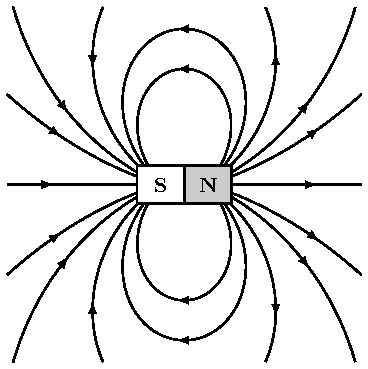
\includegraphics[width=5cm]{documents/figures/magnetic-field-lines-1.pdf}
\end{center}

\end{parts}

\question
Magnetism Station Lab: Building an Electromagnet

\textbf{Objective}: Students will construct a simple electromagnet using a battery, some wire, and a nail, and they will observe different methods of manipulating the strength of the magnet.

\begin{parts}
\part 
To build your electromagnet, start by wrapping the wire around the nail a few times and then connect the two ends of the wire to the leads of the battery. With the wire connected to the battery, can you use the nail to pick up some paperclips? If so, how many can you pick up?

\part 
Now try adding a second battery (make sure the 2 batteries are properly oriented). Can you pick up more paperclips than before or less?

\part 
Now disconnect the wire and wrap it around the nail a few more times. When you reconnect the battery, can you pick up more paperclips than before or less?
\end{parts}

\question
Magnetism Station Lab: Magnetic Field Lines

\textbf{Objective}: Students will observe the shape of the magnetic field generated by a simple bar magnet using iron filings. Note: Before you begin, make sure that the magnet is separate from the apparatus and all the iron filings are settled.

\begin{parts}
\part Place the magnet in the cylinder and shake it to spread the iron filings. Draw the shape that the iron makes around the magnet below.

\begin{solutionorbox}[4cm]
    
\end{solutionorbox}


\part
Now try pulling the magnet out most of the way so that just one end is still in the cylinder. Draw the shape of the field near the magnetic pole.

\begin{solutionorbox}[4cm]
    
\end{solutionorbox}
\end{parts}

\question
Magnetism Station Lab: Electromagnet

\textbf{Objective}: Students will observe how a coil of wire can be used as an electromagnet. Note: Before you begin, make sure the coil of wire is disconnected from the battery and the metal core is placed in the center of the coil.


\begin{parts}
\part Without connecting the battery, touch the loose metal plate to the core. Is the plate attracted to the core or not?
\part Now connect the two ends of the wire to the leads of the battery. Is the metal plate attracted to the coil/iron core or not? 
\part Take the small permanent magnet and place it near the core of your electromagnet. Which pole of the magnet is attracted to the core? Which pole is repelled?
\part Disconnect the battery, reconnect it in the opposite orientation, and repeat step 3. Has the polarity of your electromagnet changed or stayed the same?
\end{parts}


\question
Magnetism Station Lab: Faraday’s Law

\textbf{Objective}: Students will observe the effects of changing magnetic fields near conductors by waving a bar magnet around a coil of wire that is connected to a voltmeter. Note: Before you begin, make sure that your voltmeter is connected to both ends of the coil and its dial is turned to the smallest voltage scale, labeled ``200m''.

\begin{parts}
\part Take the bar magnet and wave it over the top of the coil of wire. Describe what happens to the voltmeter.
\part Now try slowly moving the North pole of the magnet in and out of the coil. Is the voltage positive or negative when you push the magnet into the coil? What about when you pull the magnet out of the coil?
\part Flip the magnet around and repeat step 2 so that the South pole is now moving in and out of the coil. Is the sign of the voltage the same as before or different?
\part Now try moving the magnet faster into the coil. Does the voltage increase or decrease? What is the maximum voltage you can achieve?
\end{parts}

\question
Magnetism Station Lab: Floating Magnet Tower

\textbf{Objective}: Students will observe the interactions between permanent magnets by changing the polarity of individual magnets on a floating magnet tower. Note: Before you begin, make sure that the tower is setup so that none of the magnets are stuck together (all are repelling their neighbors).

\begin{parts}
\part 
Try taking one of the magnets off the top of the tower. What happens to the rest of the magnets on the tower?

\part 
Now flip the magnet that you have removed upside-down and place it back on the tower. Does the magnet still float? Describe what happens to the rest of the tower.

\part 
Now take all the magnets off the tower and arrange them so that all but one of the magnets are stuck together. Place the magnets back on the tower so that the individual magnet is floating on top of the rest. Is the tower taller or shorter than when you started? What configuration makes the tower the tallest?
\end{parts}

\end{questions}

\clearpage


\subsection{Other}

\begin{questions}
\question
Magnets are categorized as magnetic dipoles. What is meant by \textit{dipole}?

\begin{randomizechoices}
    \correctchoice That a bar magnet has two poles.
    \choice That a bar magnet has one pole.
    \choice That a bar magnet has no poles.
    \choice That a bar magnet has infinitely many poles.
\end{randomizechoices}

\question
What are the labels of the poles of a bar magnet?

\begin{randomizechoices}
\choice North only
\choice North, south, east, and west
\choice East and west
\CorrectChoice North and south
\end{randomizechoices}

\question
What do you get when you cut a bar magnet in half?

\begin{randomizechoices}
\choice One magnet with two south poles, and one magnet with two north poles.
\choice Two objects that are not magnetic anymore.
\choice It’s impossible to cut a magnet in half.
\CorrectChoice Two magnets, each with a north and south pole.
\end{randomizechoices}

\question
True or False? Earth generates a magnetic field which surrounds it.

\begin{randomizechoices}[norandomize]
    \correctchoice True
    \choice False
\end{randomizechoices}

\question
The south geographic pole of Earth (in Antarctica) is near what type of \textit{magnetic} pole?

\begin{randomizeoneparchoices}
    \correctchoice north
    \choice south
    \choice east
    \choice west
\end{randomizeoneparchoices}


\question
What type of \textit{magnetic} pole is close to Earth's north \textit{geographic} pole (near Alaska)? 

\begin{randomizeoneparchoices}
\choice north
\CorrectChoice south
\choice east
\choice west
\end{randomizeoneparchoices}

\question
The \textit{magnetic} pole of Earth that is close to the \textit{geographic} South Pole is a\\ magnetic \fillin Pole.

\begin{randomizechoices}
\CorrectChoice North
\choice South
\choice East
\choice West
\end{randomizechoices}

\question
The \textit{magnetic} North Pole of Earth is close to the \textit{geographic} \fillin Pole.

\begin{randomizechoices}
\choice North
\CorrectChoice South
\choice East
\choice West
\end{randomizechoices}

\question
The \textit{magnetic} South Pole of Earth is close to the \textit{geographic} \fillin Pole.

\begin{randomizechoices}
\CorrectChoice North
\choice South
\choice East
\choice West
\end{randomizechoices}

\question
One way to visualize magnetic field lines around a magnet is by\ldots 

\begin{randomizechoices}
\choice using certified electromagnetic goggles.
\choice attracting or repelling the magnet with a second magnet.
\CorrectChoice sprinkling iron filings around the magnet.
\choice brushing the magnet with glow-in-the-dark liquid and turning off the lights.
\end{randomizechoices}

\question
Besides magnets, what other thing creates a magnetic field?

\begin{randomizechoices}[norandomize]
\choice Water.
\choice The gravitational force.
\CorrectChoice electric current (i.e., moving charges)
\choice Nothing. Only magnets can create magnetic fields.
\end{randomizechoices}

\clearpage

\question
Where were the first known magnets discovered?

\begin{randomizechoices}
\choice Houston, TX
\CorrectChoice Magnesia (present-day western Turkey)
\choice London, England
\choice The North Pole
\end{randomizechoices}

\question
Suppose that equal parts of sand and iron powder are mixed together in a glass petri dish. What happens when a magnet is placed next to one side of the dish?

\begin{randomizechoices}
\CorrectChoice Magnet attracts the iron only
\choice Magnet attracts the sand only
\choice Magnet attracts both the sand and the iron
\choice The magnet attracts the iron and repels the sand
\end{randomizechoices}

\question
In which direction do magnetic field lines from a bar magnet flow?

\begin{randomizechoices}
\choice South to North
\choice North to East
\CorrectChoice North to South
\choice South to West
\end{randomizechoices}

\question
What is electric current?

\begin{randomizechoices}
\choice a current of water
\CorrectChoice electric charges that are moving
\choice directional field lines around a magnet
\choice the atoms that make up a metal wire
\end{randomizechoices}

\question
The SI units for electric current, amperes (A), are equivalent to which other units?

\begin{randomizechoices}
\CorrectChoice C/s
\choice e/s
\choice $-$e/s
\choice C/$\mathrm{s^2}$
\end{randomizechoices}

\question
The electrons in a straight wire flow downwards. In which direction does electric current flow?

\begin{randomizeoneparchoices}
\CorrectChoice up
\choice down
\choice $\bigodot$
\choice $\bigotimes$
\end{randomizeoneparchoices}

\question
The current in a straight wire flows to the right. In which direction do electrons flow?

\question
What is the purpose of the right-hand rule?

\begin{center}
\begin{minipage}{0.3\textwidth}
\centering
    \begin{tikzpicture}
        \draw[ultra thick,->] (0,-2) -- ++(0,3.5) node[above] {$I$};
        \begin{scope}[rotate around x=50]
            \draw[red,very thick,->] (0,0) arc (90:280:1);
        \end{scope}
        \begin{scope}[yshift=2mm,rotate around x=50]
            \draw[red,very thick,->] (0,0) arc (90:283:1.6);
        \end{scope}
        \begin{scope}[yshift=4mm,rotate around x=50]
            \draw[red,very thick,->] (0,0) arc (90:286:2.2);
        \end{scope}
        \node[red] at (1.3,-0.5) {$\vec{B}$};
    \end{tikzpicture}
\end{minipage}%
\hspace{1em}
% \begin{minipage}{0.3\textwidth}
%     \centering
%         
\includegraphics[width=3.6cm]{documents/figures/Unit10_RightHandRule.jpeg}
% \end{minipage}
\end{center}

\begin{randomizechoices}
\choice to show the direction of gravity
\CorrectChoice to show the direction of magnetic field around a current-carrying wire
\choice to show the direction of current between two magnets
\choice to show the direction of magnetic field between two magnets
\end{randomizechoices}

\question
What is the direction of the magnetic field when the current is

\begin{center}
    $\bigodot I$
\end{center}

\begin{randomizechoices}
\choice {$\circlearrowright$}
\CorrectChoice {$\circlearrowleft$}
\choice $\bigodot$
\choice $\bigotimes$
\end{randomizechoices}

\clearpage
\question
What is the direction of the magnetic field when the current is

\begin{center}
    $\bigotimes I$
\end{center}

\begin{randomizechoices}
\CorrectChoice {$\circlearrowright$}
\choice {$\circlearrowleft$}
\choice $\bigodot$
\choice $\bigotimes$
\end{randomizechoices}

\question Current in a wire flows to the left, as shown by the figure. What is the direction of the magnetic field in the region \textit{above} the wire?

\begin{center}
\begin{tikzpicture}
\draw[ultra thick,<-] (0,0) node[left]{$I$} -- ++(5,0);
\begin{scope}[yshift=3mm]
    \draw[dashed] (0,0) rectangle (5,1) node[pos=0.5]{Above};    
\end{scope}
\end{tikzpicture}
\end{center}

\begin{randomizeoneparchoices}
\choice left
\choice right
\choice out of the page %$\bigodot$
\CorrectChoice into the page %$\bigotimes$
\end{randomizeoneparchoices}

\question Current in a wire flows to the left, as shown by the figure. What is the direction of the magnetic field in the region \textit{below} the wire?

\begin{center}
\begin{tikzpicture}
\draw[ultra thick,<-] (0,0) node[left]{$I$} -- ++(5,0);
\begin{scope}[yshift=-13mm]
    \draw[dashed] (0,0) rectangle (5,1) node[pos=0.5]{Below};    
\end{scope}
\end{tikzpicture}
\end{center}

\begin{randomizeoneparchoices}
\choice left
\choice right
\CorrectChoice out of the page %$\bigodot$
\choice into the page %$\bigotimes$
\end{randomizeoneparchoices}


\question Electric current flows through a vertical wire. The surrounding magnetic field goes into and out of the page as shown below. In what direction do \textbf{ELECTRONS} through the wire flow?

\begin{center}
\begin{tikzpicture}
    \draw[ultra thick] (0,0) node[below] {down} -- ++(0,3) node[above] {up} ; 
    \foreach \i in {0,0.5,...,1.5}
        \foreach \j in {0.5,1.0,...,2.5}
      {
        \begin{scope}[xshift=-2cm]
            \node at (\i,\j) {$\otimes$};
        \end{scope}
        \begin{scope}[xshift=0.5cm]
            \node at (\i,\j) {$\odot$};
        \end{scope}
      }
\end{tikzpicture}
\end{center}

\begin{randomizeoneparchoices}
    \correctchoice up
    \choice down
    \choice out of the page
    \choice into the page
\end{randomizeoneparchoices}

\clearpage

\vspace{1em}

\hrule\hrule

\begin{EnvUplevel}
\textbf{Questions \ref{JAlbal} through \ref{JxMpCM} are OPTIONAL and are worth EXTRA CREDIT.} To get full credit, show all your work on a sheet of paper, express your answer with correct units, and box your answer.
\end{EnvUplevel}

\question \label{JAlbal}
A wire carries 7.0 amperes of electric current. What is the magnetic field strength 4.5 centimeters outside the current-carrying wire? %Answer: 

\begin{solution}
    \SI{3.1e-5}{T}
\end{solution}

\question
The magnitude of the magnetic field at a point outside a current-carrying wire is shown below. Calculate the distance, in meters, of the point above the wire.

\begin{center}
    \begin{tikzpicture}
        \draw[ultra thick,->] (0,0) -- (3,0) node[right] {$\SI{12}{A}$};
        \draw[dashed] (1.5,0) -- ++(0,0.9);
        \node[red] at (1.5,1) {$\bigodot$}; \node[black,right=4pt] at (1.5,1) {\SI{8e-7}{T}};
    \end{tikzpicture}
\end{center}

\begin{solution}
    3.0 meters
\end{solution}

\question
The magnetic field strength 3 millimeters outside a current-carrying wire is \num{5e-4} tesla. Calculate the electric current through the wire.

\begin{solution}
    \SI{7.5}{A}
\end{solution}

\begin{EnvUplevel}
    \textbf{Questions \ref{LhsqrR} and \ref{JxMpCM} are in reference to the magnetic field equation:}
\end{EnvUplevel}

\begin{equation*}
    B = \frac{\mymu_0 I}{2\pi r}
\end{equation*}

\question \label{LhsqrR}
Solve the equation algebraically for distance. Show all your steps.

\question \label{JxMpCM}
Solve the equation algebraically for electric current. Show all your steps.


\question
What is the magnetic field strength at a distance of 3 m from a wire carrying a current of 2 A?

\begin{randomizechoices}
\CorrectChoice $1.3 \times 10^{-7}$ T
\choice $6.7 \times 10^{-6}$ T
\choice 6 T
\choice 5 T
\end{randomizechoices}

\question
What is the magnetic field strength at a distance of 0.05 m from a wire carrying a current of 7.3 A?

\begin{randomizechoices}
\choice $9.1 \times 10^{-5}$ T
\CorrectChoice $2.9 \times 10^{-5}$ T
\choice 0.05 T
\choice 7.3 T
\end{randomizechoices}


\question
What is a magnetic field?

\begin{randomizechoices}
\choice a field of magnets
\CorrectChoice directional lines around a magnetic material that indicate the direction and magnitude of the magnetic force
\choice a material or object that produces a magnetism
\choice part of a magnet that exerts the strongest force on other magnets or magnetic material
\end{randomizechoices}
\end{questions}

\end{document}




\subsubsection{North and South Pole}

\subsubsection{Two Magnets Attract or Repel}

\subsubsection{Classifying Materials as Magnetic or Nonmagnetic}

\subsection{Magnetic Fields}

\subsubsection{Magnetic Fields Around Magnets}

\subsubsection{Visualizing Magnetic Field Loops}

\subsubsection{Predicting Attraction or Repulsion by Field Lines}

\subsubsection{Magnetic Field Strength by Field Lines}

\subsection{Compass}

\subsubsection{How a Compass Points in the Direction of the Magnetic Field}

\subsubsection{Earth's Magnetic and Geographic Poles}

\subsection{Electromagnetic Fields}

\subsubsection{Magnetic Fields and Moving Charges}

\subsubsection{Magnetic Fields around Current Carrying Wires}

\subsubsection{Representing Magnetic Fields Into and Out of the Page}

\subsection{Electromagnetic Induction}

\subsubsection{Changing Magnetic Fields and Induced Electrical Currents}

\subsubsection{Faraday's Law}

\clearpage

\subsection{Electromagnet}

\subsubsection{How Electromagnets Generate Magnetic Fields}

\subsubsection{Making an Electromagnet Stronger}

\subsection{Transformers}

\subsubsection{Diagram of a Transformer}

\subsubsection{Changing Voltage while Conserving Energy}

\subsubsection{Stepping Voltage Up or Down}

\subsection{Generators and Motors}

\subsubsection{Converting Mechanical to Electrical Energy}

\subsubsection{Inducing More or Less Current in a Generator}

\subsubsection{Moving Charge in an External Magnetic Field}

\subsubsection{Construction and Operation of a Motor and Generator}

\subsubsection{Changing the Rotational Speed of a Motor}